\originalchapter{22.02 2011 年期中卷}
题源: 2011年3月17日 Mid-Term Exam, 2012课程的历史练习材料. 官方答案中有测量简并与数值近似问题, 本章分别更正, 不把网页错误的 Final 栏名称当作真正期末卷.
\begin{exercise}\label{ex:2202-e2011-1}
原题 1 (八组). (1) 波函数能给系统哪些信息? (2) 先测动能再测动量, 第二次结果随机吗? (3) SEMF Coulomb 项描述什么? (4) $\psi(y)=A\e^{-\ii\pi y}$ 的动量结果、概率、物理情形? (5) 波函数何时为能量本征函数? (6) 下列态哪些合法: $|l=3,m_z=-4\rangle$, $|l=4,m_x=3,m_z=-2\rangle$, $|l=4,m_x=3\rangle$? (7) 用 E 与 V 说明束缚. (8) Q 是否独自确定核反应自发发生?
\end{exercise}
\begin{solution}
(1) 对给定可观测量计算所有结果概率和均值, 包括位置但不限于位置. (2) 一般仍随机, 因自由动能 $p^2/(2m)$ 对 $\pm p$ 简并. 例如测后 cos 态有两个动量各1/2. 官方答案用``先测动量再测动能''解释的是反向顺序, 不能回答原问. (3) 质子间 Coulomb 排斥减少结合, 标度 $Z(Z-1)/A^{1/3}$. (4) $p_y=-\pi\hbar$ 唯一, 广义自由定动量态沿负 y 传播. (5) $H\psi=E\psi$, 封闭定 H 下只获得整体相位, 是定态. (6) 只有第三项合法; 第一 $|m|>l$, 第二同时给不对易的两个非平凡分量确定值不合法. (7) 对外势趋0的有限阱, 负 E 且波函数正规可积是束缚条件; 不能仅凭局部 E<V 就断定全体系束缚. (8) 正 Q 只表能量许可, 还需守恒与矩阵元, 势垒会抑制率.
\end{solution}
\begin{exercise}\label{ex:2202-e2011-2}
原题 2. (a) 同 z 轴经典转动对易吗, x 与 y 转动呢? (b) 用小角 $R_n(\theta)=1-\ii\theta L_n/\hbar$ 判断量子转动对易. (c) 比较先 y 再 x 与先 x 再 y 的差, 能表示为转动吗? (d) 若 $R_x(\theta)\psi=\psi$, 是否为 $L_x$ 本征态? (e) $\psi=\phi_{-2}/\sqrt6+\phi_0/2+\sqrt{7/12}\phi_1$, 各 $\phi_m$ 是 $L_x$ 归一态, 测0概率及均值?
\end{exercise}
\begin{solution}
(a) 同轴对易, 不同轴一般不对易, 特殊零角等例外. (b) 不同轴的生成元不对易, 小角转动仍不对易. (c) $R_x(\theta)R_y(\varphi)-R_y(\varphi)R_x(\theta)=-\ii\theta\varphi L_z/\hbar+O(\theta^2\varphi,\theta\varphi^2)$, 等于 $R_z(\theta\varphi)-I$ 的最低阶. (d) 若对任意足够小 $\theta$ 都不变, 求导得 $L_x\psi=0$, 是零本征态. 若只对单个角不变, 如 $\theta=2\pi$ 的整数自旋, 不能推断单一 $L_x$ 态. 原题需要这个量词条件. (e) P(0)=1/4, $\langle L_x\rangle=(-2/6+7/12)\hbar=\hbar/4$.
\end{solution}
\begin{exercise}\label{ex:2202-e2011-3}
原题 3. $^{131}_{63}$Eu 质量121919.966 MeV, $^{130}_{62}$Sm 质量120980.755 MeV, $m_pc^2=938.272$ MeV, $\hbar c=197$ MeV fm, $e^2/(\hbar c)=1/137$, $r_0=1.2$ fm. (a) 是否预计稳定? (b) Eu$\to$Sm+p 的 Q. (c) 以 Q 为 proton 动能, 求 $f=v/R$. (d) 接触 $R=R_{\rm Sm}$ 的 Coulomb 势及外转折点 $R_c$. (e) 方垒 $V_H=V_C(R)/2,L=(R_c-R)/2$ 的 T. (f) 衰变率及半衰期.
\end{exercise}
\begin{solution}
官方估算路线, 数字独立复算. (a) N=68,Z=63, 对重于轻核的区域明显 proton 过多, 预计不稳定. (b) 题设质量作为同一口径核质量, Q=$0.939$ MeV. 不混入其他原子质量表. (c) $R=6.079$ fm, $v=c\sqrt{2Q/m_p}=0.0447c$, $f\simeq2.208\times10^{21}$ s$^{-1}$. (d) $C=62\hbar c/137=89.15$ MeV fm, $V_C(R)=14.67$ MeV, $R_c=C/Q=94.94$ fm. (e) $V_H=7.333$ MeV,L=44.43 fm,$\kappa=0.5560$ fm$^{-1}$. 用厚垒前因子 $16Q(V_H-Q)/V_H^2$ 得 $T\simeq6.20\times10^{-22}$. (f) $\lambda=fT\simeq1.37$ s$^{-1}$, $t_{1/2}\simeq0.506$ s. 若沿用课堂 $4\e^{-2\kappa L}$, 将得另一量级值; 舍入指数会显著变化. 实际还含质子轨道离心势垒、预形成和真实势形, 不把此粗估当作精确核数据.
\end{solution}
\begin{exercise}\label{ex:2202-e2011-4}
原题 4。图左给五个一维波形A--E的实部，右给四个分段势与能线1--4，区域标为I--V。每个波形应与哪一幅势能图匹配？一幅势能图可以匹配多个波形。逐一区分束缚态、左右入射的散射边界条件，以及各区的振荡、波长和指数尾。
\end{exercise}
\begin{center}
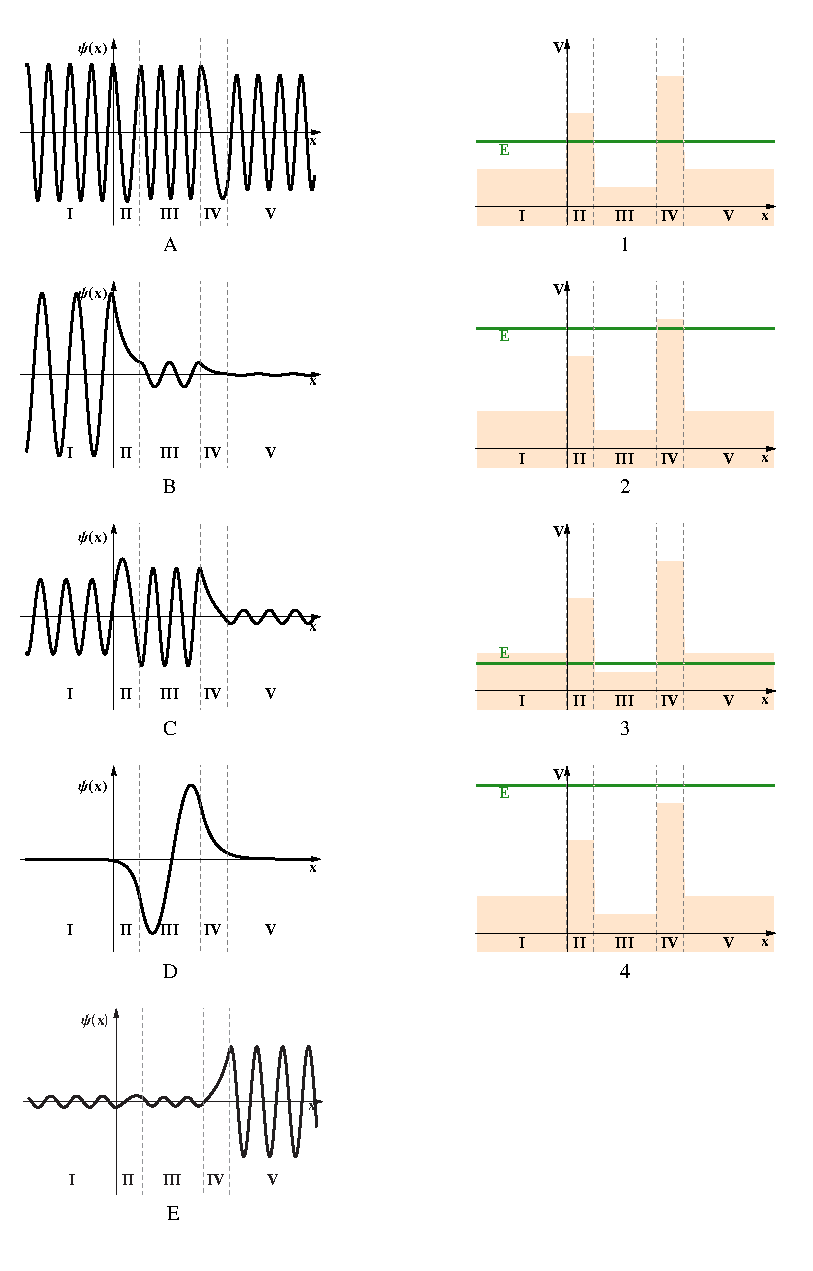
\includegraphics[width=.79\linewidth]{figures/ocw-exam-2011-q4.pdf}\\
{\small 原题图：Paola Cappellaro，MIT 22.02 Spring 2012 OCW，2011期中题卷第3页，裁取矢量图。}
\end{center}
\begin{solution}
官方定性答案为 A--4、B--1、C--2、D--3、E--2. A 的局部波数均为实; B 两垒禁阻; C只有最高垒禁阻; D在中央阱束缚且两侧可积; E从右入射, 穿过最高垒后振幅变小, 相同能量却不同散射边界条件. 禁阻有限区允许增长与衰减指数的组合, 单看一个区的增长并不说明态发散; 只有无穷远处必须删掉非物理增长项. 源图为定性曲线, 不给可复原的数值波形, 因此不从草图振幅算截面.
\end{solution}
